\documentclass{article}
\usepackage[utf8]{inputenc}
\usepackage{graphicx}
\usepackage{caption}
\usepackage[english]{babel}

\usepackage{amsmath,amssymb}
\usepackage{a4wide}
\usepackage{tikz}
\usetikzlibrary{calc}
\title{Description Capita Selecta}
\author{Omar Richardson}
\date{March 2015}
\let\oldhat\hat
\let\oldtil\tilde
\DeclareMathOperator{\diag}{diag}
\renewcommand{\vec}[1]{\mathbf{#1}}
\newcommand{\gvec}[1]{\boldsymbol#1}
\renewcommand{\tilde}[1]{\oldtil{\mathbf{#1}}}
\newcommand{\eps}{\varepsilon}
\newcommand{\bigo}[1]{\mathcal{O}\left(#1\right)}
\begin{document}

\maketitle

\section{Abstract}
Crowd dynamics is an emerging field of research. With more computational power and algorithms available, realistic crowd simulations become better and better. When desiring to model a crowd, several dependable modelling options are available. Some models employ stochastic differential equations to model the movements of agents as Brownian motions. Other models represent the agents as occupied cells on a grid.
\ \\
These ways of modelling has proven to work well for small crowds. When crowds become dense, other options become available as well. One of these options is to combine both a global as a local approach in the model, where the global approach models the crowd as a fluid, and the local approach models agents as individual agents. Using the right simulation architecture, this way of modelling is able to handle crowds with a large number of agents at a relatively low computational cost.

\ \\
The goal of this capita selecta is to implement this method and check its performance in the case of a large crowd in need of evacuation. If time permits it, we will make a comparison to other models in order to evaluate performance.

\newpage
\section{Implementation overview}
The simulation of this model is composed of several modules. These modules will be implemented separately. This will enable us to swap or upgrade modules without having to adapt the rest, in order to keep the simulation improvable and maintainable.
\begin{enumerate}
\item \textbf{Geometry}\\
This part models the scenario in which the agents are placed, the obstacles present, and the exits they are headed to.
\item \textbf{Global planner}\\
This module determines the destinations of the agents. From these destinations and the geometry, it determines the desired speed and direction of every agent.
\item \textbf{Conversion of agents to fluid model}\\
This module is responsible for translating the position and speed of the agent to a continuous representation (limited to a grid). The resulting flow field can be used for determining global behaviour of the agents.
\item \textbf{Fluid flow solver}\\
This module is responsible for determining the global direction of the agents. Every agent is confined this direction in a certain degree. The denser the crowd, the less influence one agent has over its direction.
This module also contains the incompressibility constraint to prevent agents from colliding.
\end{enumerate}
The model will be implemented in Python. Motivation behind this language is that it has dependable scientific computing libraries available, like \texttt{numpy} and \texttt{scipy}. It also has the advantage of object oriented structure, which will make working with agents on a local level more manageable.
\newpage
\section{Geometry}
This section will elaborate on the implementation of the geometry.
\subsection{Summary}
The geometry consists of a scene filled with multiple obstacles. The scene is the domain of calculation. It is modelled as a rectangle, surrounded with walls and exits. Within this domain, agents are spawned, trying to make their way to the exit while dodging the obstacles (and each other). an agent will be eliminated once he has made his way to the exit.

\subsection{Structure}
The geometry is divided into a computational component and a visual component. The computational component handles the computations of the next time step of the scene. The visual component acts separately and displays the geometry (and the agents) at every time step. This part can be suppressed to increase simulation capacity.

\subsection{Obstacles}
The scene can be filled with an arbitrary number of objects, provided that all agents spawned are able to reach the exit given their initial location. The objects have a rectangular shape. This choice is motivated by their relative ease in modelling and calculating. In addition, rectangular objects can easily be aggregated to more general shapes.
\ \\
A scene contains both an entrance and an exit. The entrance is modelled as an obstacle with a certain \underline{inflow} of agents (this allows us to imitate a PDE-like boundary condition) and the exit is modelled as a penetrable obstacle. By default, a scene is surrounded by objects functioning as walls. Whenever an exit or entrance is defined, it replaces the walls.
\subsection{Agents}
The agents are modelled as agents with a position and a velocity. The position and velocity are stored locally for now. We keep in mind that storing and manipulating this information on a global level will improve computational speed.
The agents have a maximum speed which varies among them.

\ \\
The agents are displayed in the geometry by colored circles. Optionally, it is possible to display the agents as directed triangles, to indicate their movement direction. This, again, has a \underline{higher computational cost}.
\newpage
\section{Planner - Naive}
This section describes the initial planner module implemented.
\subsection{Summary}
The planner has the objective of planning a path for every agent to follow that will lead him to his goal. This path has to respect the obstacles, but can be ignorant of other agents, since the fluid solver will account for that.

\ \\
A \emph{path} is modelled as a sequence of sub-paths, straight line segments. This makes the path piecewise linear.
The path from an agents position to the exit is determined by computing the corresponding line segment and \underline{iteratively} dodging the obstacles in the way until a collision-free path has been established. This path is then imposed on the agent.
An agents \emph{goal} is a special kind of obstacle which can be entered. The distance from the agent to the goal is defined as the Euclidean distance between a point (the agent position) and a set (the rectangular goal).

\ \\
The planner computes the line segment corresponding to the aforementioned distance and detects if any obstacles \emph{hinder} the path. These obstacles are examined and the planner tries to find a sub-path avoiding the obstacles that deviates as little as possible from the original path. After determining this sub-path, the planner goes on to repeat the process starting from the end of the new sub-path. It does so until a new location has been found and \underline{errors} if no path has been found after too many iterations.
\subsection{Determining hindering obstacles}
A path is hindered by an obstacle if that obstacle and the path have common points \underline{Figure}. Because sub-paths are line segments, they can be expressed as a simple linear parameter equation. The rectangular obstacles are solely determined by two points in the plain $\mathbb{R}^2$. Determining a hindering objects then can be reduced to finding a parameter for which the parameter equation of the sub-path lies between the points of the object.

\ \\
There are several ways to solve this problem. Because it has to be solved frequently, we use a solution that can be vectorized to solve simultaneously for large numbers of agents.
We represent the line segment with coordinates $r_1$ and $r_2$. The parameter equation becomes $r_1 + \lambda(r_2 - r_1)$ for $\lambda \in [0,1]$. We represent the obstacle with points $a_1$ and $a_2$ (\underline{Figure}). We perform several translations on the line segment (and obstacle) to reduce the obstacle to the unit square with respect to the Manhattan norm. This reduces our problem to finding a parameter $\lambda$ such that our parameter equation has a Manhattan norm of 1. In detail, the following happens:
\begin{itemize}
\item The line segment is translated with vector $-\frac{(a_0+a_1)}{2}$. This centers the obstacle.
\item The line segment is scaled with factor $(a_0-a_1)$. This transforms the (rectangular) obstacle to the unit square with respect to the infinity-norm
\item The line segment is rotated with respect to the origin over an angle of $\frac{\pi}{4}$. This transforms the obstacle to the unit square with respect to the 1-norm.
\end{itemize}
Note that these computations are not actually performed on the obstacle itself, only on the line segments.
\ \\
The result is a translation of the line segment as in Figure \ref{}. Now we solve 
$$||\hat{r}_1 + \lambda(\hat{r}_2-\hat{r}_1)||_1<1$$
which is equivalent to 
$$\sum_{j\in\{x,y\}}|\hat{r}_{1j} + \lambda(\hat{r}_{2j}-\hat{r}_{1j})|<1.$$
This resulting function is convex and piecewise linear, resulting in an accurate numerical solution to the inequality
\ \\
If such a $\lambda\in[0,1]$ is found, the obstacle hinders the sub-path. Otherwise, the sub-path is free.
\subsection{Dodging obstacles}
We solve the pathplanning problem by converting objects into a graph and using the \texttt{networkx} library \cite{networkx} to find the shortest path\dots
\newpage
\section{Continuum aspects}
This section will elaborate on the continuum part of the implementation; converting the agents to a continuum and computing its properties.
\subsection{Overview}
The \underline{continuum solver} uses the following partial differential equation, based on the continuity equation for mass but adapted with a pressure term.
\begin{equation}\label{eq:pde}
\frac{\partial \rho}{\partial t} =-\nabla \cdot(\rho{v}) + \nabla \cdot (\rho\nabla p)
\end{equation}
with scalar density field $\rho(x,y,t)$, vector velocity field $v(x,y,t) = \begin{pmatrix}v_x\\v_y\end{pmatrix}$ and scalar pressure field $p(x,y,t)$.

\ \\
To utilise our fluid flow solver, we need a global representation of the agents. The agents' individual mass and velocity has to be converted to a global density, velocity and pressure. In this implementation, we choose to define a grid of cells over the scene. In each cell, we compute a numerical estimate for each field. Both the density and the velocity of a given cell are interpolated from the agents nearby the cell. Then, using these two fields, we numerically compute the next time step of the pressure and the velocity in \eqref{eq:pde}. Finally, we use these two fields to restrict the motion of the agents.

\ \\
Our fluid solver influences the agents in two ways: 
\begin{itemize}
\item Swarm behaviour
\item Incompressibility
\end{itemize}
\subsubsection{Incompressibility Constraint}
Our incompressibility imposes some restrictions on the density and the velocity. We assume a maximum density $\rho_{\max}$. Wherever our density $\rho(x)$ reaches $\rho_{\max}$, the scene is locally saturated, and the agents have to divert from their path. 

\ \\
\underline{Using variational calculus} we obtain that the optimal $v$ respecting $v_{\max}$ equals $$v = v_{\max}\frac{v-\nabla p}{||v-\nabla p||}.$$
under the constraints that 
\begin{align}
\label{eq:comp}
p>0 \texttt{ OR } \rho=\rho_{\max}\\
p>0 \implies \nabla\cdot v=0
\end{align}
Note that \eqref{eq:comp} implies that $\rho$ and $p$ are complementary variables, i.e. that $\rho(x)p(x)=0$ for all $x$.
\subsubsection{Swarm behaviour}
The solver computes the velocity field of the crowd on a grid. This field influences the individual speed of the agents. When the density in an agents neighbourhood becomes higher, his velocity will converge to the velocity of the crowd. The actual velocity $v_{a_i}$ of agent $a_i$ (located at $(x_{a_i},y_{a_i})$) becomes the average of his desired velocity $\bar{v}_{a_i}$ and the crowds velocity $v(x_{a_i},y_{a_i},\cdot)$, weighted to the local density:
\begin{equation}
	v_{a_i} = \left(1-\frac{\rho(x_{a_i},y_{a_i},\cdot)}{\rho_{\max}}\right)\bar{v}_{a_i}+\frac{\rho(x_{a_i},y_{a_i},\cdot)}{\rho_{\max}}v(x_{a_i},y_{a_i},\cdot)
	\label{eq:dens_velo}
\end{equation}


\subsection{Discretization}
We desire a numerical approximation of $\rho$, $p$ and $v$. To obtain this, we first discretize our domain and our equation. We define a grid of $(N_x,N_y)$ cells, where every cell has a size of $h_x\times h_y$. Our complete scene has dimensions $N_xh_x\times N_yh_y$. 
\ \\
We discretize our scalar and vector fields corresponding to the grid. We index the cells (and the fields) from the bottom left, corresponding with the Carthesian coordinate system in the scene. This is illustrated in Figure \ref{fig:indexing}.
\begin{figure}
	\centering
	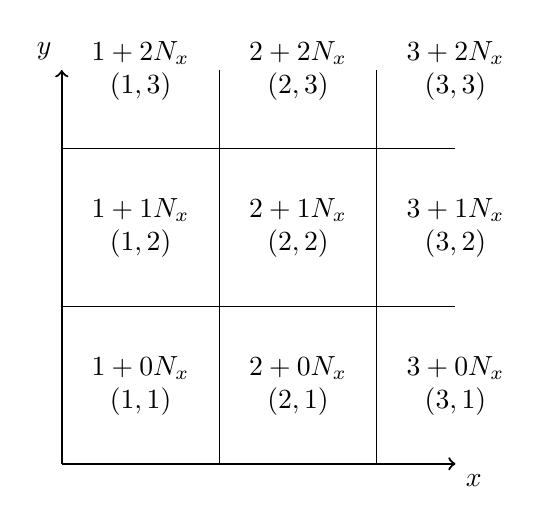
\begin{tikzpicture}
		\draw[step=2cm,black,thin] (0,0) grid (5,5);
		\draw[thick,->] (0,0) -- (5,0) node[anchor=north west] {$x$};
		\draw[thick,->] (0,0) -- (0,5) node[anchor=south east] {$y$};
		\foreach \x in {1,2,3}
			\pgfmathparse{\x*2-1}
			\edef\cx{\pgfmathresult}
			\foreach \y in {1,2,3}
				\pgfmathparse{\y*2-1}
				\edef\cy{\pgfmathresult}
				\pgfmathparse{int(\y-1)}
				\edef\ym{\pgfmathresult}
				\draw (\cx cm,\cy cm) node[anchor=center] {$\begin{matrix}\x+\ym N_x\\ (\x,\y)\end{matrix}$};
	\end{tikzpicture}
	\captionof{figure}[Caption]{Orientation of the coordinates and fields in the scene, with corresponding $\left(\begin{matrix}\text{1D} \\ \text{2D} \end{matrix}\right)$ cell indexing of the scene. The 1D notation is used to orient corresponding vectors and matrices, while the 2D notation is used for legibility and elementwise computations}
	\label{fig:indexing}
\end{figure}
This way, we discretize our fields to vectors $\gvec{\rho}^n,\vec{v_x}^n,\vec{v_y}^n, \vec{p}^n\in\mathbb{R}^{N_xN_y}$ for any time step $n\in\mathbb{N}$. The relation between a field $u$ and its discrete representation $\vec{u}^n$ is defined as
$$\vec{u}^n_{(i,j)} = u((i-0.5)\Delta x,(j-0.5)\Delta y,n\Delta t)$$
This way the entries of vector $\vec{u}$ are approximations at the centre of the corresponding cells.
\ \\
So for any discrete scalar field $\vec{u}$, the value in cell $(i,j)$ is denoted as $\vec{u}_{i+(j-1)N_x}$. To increase legibility, we introduce a corresponding notation for indexing the scalar field in $(i,j)$:
\begin{equation}
	\vec{u}_{(i,j)}:=\vec{u}_{i+(j-1)N_x}
\end{equation}
\subsection{Interpolation}
Before being able to discretize our density and velocity fields, we first need to interpolate them from individual agent positions. Let the scene contain $n$ agents, $a_1,\dots,a_n$, located at position $(x_{a_i},y_{a_i})$.
\ \\
The agents are modelled as Lagrangian particles. This means the agents have no volume, but their mass and velocity are concentrated into a single point.
In this implementation, we assume equal mass for all agents: $m_{a_i}=m = 1\ \forall i$. 
We convert an agents mass to a density by convolving with a two-dimensional Gaussian kernel $\phi(x,y)$ defined as 
\begin{equation}
	\label{eq:gaussian}
	\phi(x,y)=A \exp\left(-\left(\frac{x^2}{2\sigma_x^2}+\frac{y^2}{2\sigma_y^2}\right)\right)
\end{equation}
\emph{Currently, we are in the process of finding suited values for $A$, $\sigma_x$ and $\sigma_y$.}

\ \\
Let $\delta_{(x_0,y_0})$ be the Dirac distribution with value $\infty$ in $(x_0,y_0)$ and 0 everywhere else. Let $f*g$ be the convolution of $f$ and $g$. 
\ \\
Let agent $a_i$ be in location $(x_{a_i},y_{a_i})$ at time $t$. Then the density contribution $\rho_{a_i}(x,y)$ and velocity contribution $v_{a_i}(x,y)$ become
\begin{align}
	\rho_{a_i}(x,y) = m\delta*\phi\\
	v_{a_i}(x,y) = \begin{pmatrix}v_{a_i,x}\\v_{a_i,y}\end{pmatrix}\delta*\phi
\end{align}
Since $\phi$ is rotation symmetric, it can be expressed in polar coordinates:
\begin{align}
	r = \sqrt{\frac{x^2}{2\sigma_x^2}+\frac{y^2}{2\sigma_x^2}}\\
	\phi(r) = A\exp\left(-r^2\right).
\end{align}
We use a approximation of the Gaussian kernel called the Wendland-kernel \cite{violeau12}. This kernel is defined as follows:
\begin{equation}
	\label{eq:wendland}
	f_W(r) = \begin{cases}
				\left(1-\frac{r}{2}\right)^4(1+2r)& 0\leq r \leq 2\\
				0 & 2 < r 
			\end{cases}
\end{equation}
This approximation has some nice computational properties in comparison to other Gaussian approximation. We can reveal them by rewriting the expression to 
\begin{equation}
	f_W(r) = \max\left\{1-\frac{r}{2},0\right\}^4(1+2r)
\end{equation}
which is a single case function requiring only addition, multiplication, and a $\max$ function. This provides a welcome computational benefit, since a kernel convolution is a common operation in this implementation.

\ \\
To find the total density and total velocity in the cell centres for each cell, we sum over the densities and velocities of the agents in the (up to 8) neighbouring cells. This method is equivalent to the particle-in-cell method as described in \cite{zhu13}

\subsection{Scheme}
\label{sec:scheme}
To discretize our partial differential equation we use a second order central difference scheme. So for scalar field $u$ we have the following gradient approximation:
\begin{align*}
\nabla u=\begin{pmatrix}\dfrac{\partial u}{\partial x}\\\dfrac{\partial u}{\partial y}\end{pmatrix}
=\begin{pmatrix}\dfrac{\vec{u}_{(i+1,j)}-\vec{u}_{(i-1,j)}}{2h_x}\\\dfrac{\vec{u}_{(i,j+1)}-\vec{u}_{(i,j-1)}}{2h_y}\end{pmatrix}+\bigo{h^2}.
\end{align*}
and for vector field $w$ we define the divergence approximation accordingly:
\begin{equation}
\nabla\cdot w=\dfrac{\partial w}{\partial x}+\dfrac{\partial w}{\partial y}=\dfrac{\vec{w}_{(i+1,j)}-\vec{w}_{(i-1,j)}}{2h_x}+\dfrac{\vec{w}_{(i,j+1)}-\vec{w}_{(i,j-1)}}{2h_y}+\bigo{h^2}.
\end{equation}
However, if we were to discretize $\nabla\cdot(\nabla u)$ this way, computing the value at cell $(i,j)$ would require cell values from non-adjacent neigbour cells. Therefore, when computing the divergence of the gradient, we use the more compact scheme:
\begin{equation*}
\nabla\cdot(\nabla u) = \dfrac{\vec{u}_{(i+1,j)}-2\vec{u}_{(i,j)}+\vec{u}_{(i-1,j)}}{h_x^2}+\dfrac{\vec{u}_{(i,j+1)}-2\vec{u}_{(i,j)}+\vec{u}_{(i,j-1)}}{h_y^2}+\bigo{h^2}
\end{equation*}
This way, we have ensured all terms of the PDE can be computed for every cell not on the boundary.

\ \\
To discretize in time, we use the explicit Euler method. This way we only need the values of the previous time step to compute the values of the next time step. This suits our system best, because after every iteration of the fluid flow solver, the scene has changed due to individual actions of agents. Therefore previous time steps have little practical information.

\ \\
Our resulting scheme is presented below:
\begin{equation}
	\begin{split}
		\dfrac{\gvec{\rho}^{n+1}_{(i,j)} - \gvec{\rho}^{n}_{(i,j)}}{\Delta t} =
		% div(\gvec{\rho}*v)\Delta t
		&-\dfrac{\gvec{\rho}^{n}_{(i+1,j)}\vec{v}^{n}_{x(i+1,j)}-\gvec{\rho}^{n}_{(i-1,j)}\vec{v}^{n}_{x(i-1,j)}}{2h_x} \\
		&-\dfrac{\gvec{\rho}^{n}_{(i,j+1)}\vec{v}^{n}_{y(i,j+1)}-\gvec{\rho}^{n}_{(i,j-1)}\vec{v}^{n}_{y(i,j-1)}}{2h_y}\\
		%div(\gvec{\rho}*\grad \vec{p})\Delta t
		&+\frac{1}{h^2_x}\left(\frac{1}{4}(\gvec{\rho}^{n}_{(i+1,j)}-\gvec{\rho}^{n}_{(i-1,j)})(\vec{p}^{n}_{(i+1,j)}-\vec{p}^{n}_{(i-1,j)})+ \gvec{\rho}^{n}_{(i,j)}(\vec{p}^{n}_{(i+1,j)}-2\vec{p}^{n}_{(i,j)}+\vec{p}^{n}_{(i-1,j)})\right)\\
		&+\frac{1}{h^2_y}\left(\frac{1}{4}(\gvec{\rho}^{n}_{(i,j+1)}-\gvec{\rho}^{n}_{(i,j-1)})(\vec{p}^{n}_{(i,j+1)}-\vec{p}^{n}_{(i,j-1)})+ \gvec{\rho}^{n}_{(i,j)}(\vec{p}^{n}_{(i,j+1)}-2\vec{p}^{n}_{(i,j)}+\vec{p}^{n}_{(i,j-1)})\right)
	\end{split}
	\label{eq:scheme}
\end{equation}
It is suitable to express our scheme in matrices and vectors. Not only does this provide us with an efficient way to implement our scheme, it also sets us up for an efficient way of solving the PDE (as explained in Section \ref{sec:lcp})

\ \\
Before reformulating our scheme, we introduce \emph{Kronecker} products and vector gradients.
\subsubsection{Kronecker product}
Let $A \in \mathbb{R}^{m\times n}$ and $B \in \mathbb{R}^{p \times q}$. The Kronecker product $A\otimes B\in \mathbb{R}^{mp \times nq}$ is defined as
\begin{equation*}
	A\otimes B = \begin{pmatrix}
		a_{11}B &\cdots & a_{1n}B\\
		\vdots & \ddots & \vdots\\
		a_{m1}B & \cdots & a_{mn}B
	\end{pmatrix}.
\end{equation*}
The Kronecker product will prove valuable in notation and computation of our matrices.
% \subsubsection{Hadamard Product}
% Let $A \in \mathbb{R}^{m\times n}$ and $B \in \mathbb{R}^{m \times n}$. The Hadamard product $A\circ B\in \mathbb{R}^{m \times n}$ is the elementwise product of $A$ and $B$:
% \begin{equation*}
% 	A\circ B = \begin{pmatrix}
% 		a_{11}b_{11} &\cdots & a_{1n}b_{1n}\\
% 		\vdots & \ddots & \vdots\\
% 		a_{m1}b_{m1} & \cdots & a_{mn}b_{mn}
% 	\end{pmatrix}.
% \end{equation*}
% Each of the terms \eqref{eq:scheme1}, \eqref{eq:scheme1}, \eqref{eq:scheme3}, and \eqref{eq:scheme4} can be expressed separately by a combination of Kronecker products.
\subsubsection{Vector gradient}
In Section \ref{sec:scheme} we defined the discretization of the gradient. We would like to compute a gradient for every cell in the scene, even for the boundary. Therefore we surround our scene with a extra layer of cells. These virtual cells are meant to ensure the presence of 8 neighbour cells for all the cells in the scene. We fix the density and velocity in these virtual cells to 0. 
For a discrete field $\vec{u}\in \mathbb{R}^{N_xN_y}$ let the auxiliary extended field be denoted by $\vec{\tilde{u}} \in \mathbb{R}^{(N_x+2)(N_y+2)}$ defined such that:
\begin{equation}
	\vec{\tilde{u}}_{(i,j)} = \begin{cases}
		\vec{u}_{(i,j)}&\mbox{if } i \in \left\{ 1,\dots,N_x \right\},j \in \left\{ 1,\dots,N_y \right\} \\
		0&\mbox{else}
	\end{cases}.
	\label{def:gradient}
\end{equation}
Now we can define a gradient for every cell in the scene.
\begin{align*}
	\nabla_x\vec{u}_{(i,j)} &= \vec{\tilde{u}}_{(i+1,j)}-\vec{\tilde{u}}_{(i-1,j)}\\
	\nabla_y\vec{u}_{(i,j)} &= \vec{\tilde{u}}_{(i,j+1)}-\vec{\tilde{u}}_{(i,j-1)}
\end{align*}
\subsubsection{Matrix composition}
We first define two tridiagonal matrices $P_{m},Q_{m}\in \mathbb{R}^{m\times m}$
\begin{align*}
	P_{m} &= \begin{pmatrix}
		0 & -1 &  & &  \\
		1 & 0 & -1 &   &  \\
		  & 1 & \ddots & \ddots &  \\
		  &  & \ddots & \ddots &-1 \\
		 & &  & 1 & 0
	\end{pmatrix}\\
	Q_{m} &= \begin{pmatrix}
		2 & -1 &  & &  \\
		-1 & 2 & -1 &   &  \\
		  & -1 & \ddots & \ddots &  \\
		  &  & \ddots & \ddots &-1 \\
		 & &  & -1 & 2
	\end{pmatrix}
\end{align*}
Let $I_m$ be the identity matrix of rank $m$. Let $\diag:\mathbb{R}^n\rightarrow\mathbb{R}^{n\times n}$ be the operator that converts a vector $\vec{p}$ to a diagonal matrix:
\begin{equation}
	\diag(\vec{p}) = \begin{pmatrix}
		\vec{p}_1\\
		&\vec{p}_2\\
		&&\ddots\\
		&&&\vec{p}_n
	\end{pmatrix}.
	\label{def:diag}
\end{equation}
Finally we can define our scheme with two matrices for each divergence term in \eqref{eq:scheme}.
\begin{align*}
	A_x &= \frac{1}{4h_x^2}\diag(\nabla_x\gvec{\rho}^n)(P_{N_x}\otimes I_{N_y})\\
	A_y &= \frac{1}{4h_y^2}\diag(\nabla_y\gvec{\rho}^n)(I_{N_x}\otimes P_{N_y})\\
	B_x &= \frac{1}{h_x^2}\diag(\gvec{\rho})(Q_{N_x}\otimes I_{N_y})\\
	B_y &= \frac{1}{h_y^2}\diag(\gvec{\rho})(I_{N_x}\otimes Q_{N_y})
\end{align*}
Our final matrix $C$ becomes 
\begin{equation}
	C = A_x + A_y + B_x + B_y 
	\label{eq:total_matrix}
\end{equation}
\emph{I will find more suitable names for these matrices.}
\ \\
We can define a vector $\vec{b}$ to express the \underline{velocity divergence} term:
\begin{equation}
	\vec{b} = -\left( \nabla_x(\vec{v}^n_{x(i,j)}\gvec{\rho}^n_{(i,j)}) + \nabla_y(\vec{v}^n_{y(i,j)}\gvec{\rho}^n_{(i,j)})\right)
	\label{def:vector}
\end{equation}
\section{Linear complementary problem}
\label{sec:lcp}
This system is linear in both $\vec{p}$ and $\gvec{\rho}$. Combining this with the complementarity between $\vec{p}$ and $\gvec{\rho}$ we can solve this system efficiently by reformulating it to fit a linear complementarity problem (LCP).
\subsection{Definition}
For matrix $M \in \mathbb{R}^{m\times n}$ and vector $\vec{q}\in \mathbb{R}^n$, a LCP has the following general form. Find $\vec{w},\vec{z}\in \mathbb{R}^m$ such that
\begin{align}
	\vec{w}=M\vec{z}+\vec{q}\\
	\vec{w}\geq\vec{0},\vec{z}\geq\vec{0}\\
w_iz_i=0\mbox{ for all }i
\label{def:lcp}
\end{align}
Positive semidefiniteness of $M$ is a sufficient condition to solve this problem, regardless of $q$.
We choose the following expressions:
\begin{align}
	\vec{w} &= \rho_{\max}-\gvec{\rho}^{n+1}\\
	\vec{q} &= \rho_{\max}-\gvec{\rho}^n+\left(\nabla_x(\gvec{\rho}^n\vec{v}^n)+\nabla_y(\gvec{\rho}^n\vec{v}^n)\right)\Delta t\\
	\vec{z} &= \vec{p}^n\\
	M &= C\Delta t\\
	\label{eq:lcp}
\end{align}
Using these expressions, we have reformulated our scheme to an LCP.
\emph{Here should follow some analysis as to why $C$ is not far from symmetric and positive definite. I used a minimum value on $\gvec{\rho}$ which should ensure positive eigenvalues on $C$.}
\subsection{Quadratic program}
There are several ways to solve linear complementary problems. If  matrix $M$ is positive definite, LCPs can be solved by a quadratic program (QP) solver, of which there exist many. Since we asserted $M$ to be positive definite, we rewrite our LCP to a quadratic program and solve it using the Python library \texttt{cxvopt} \cite{cvxopt}.
\ \\
Any LCP of the form \eqref{def:lcp} can be rewritten to a QP as follows: Minimize $f(\vec{z})$ where
\begin{equation}
	f(\vec{z}) = \vec{z}^T\left( M\vec{z}+\vec{q} \right)
\end{equation}
with the constraints:
\begin{align}
	M\vec{z} + \vec{q}\geq\vec{0}\\
	\vec{z}\geq\vec{0}
\end{align}
Note that these constraints assert $f(\vec{z}) \geq 0$. 

\ \\
$\vec{z}$ is a solution to our LCP if and only if $f(\vec{z})=0$. Should it be that due to numerical errors no such $\vec{z}$ can be found, we still yield a satisfying\footnote{verify this} approximation by having found a minimum for $f(\vec{z})$.
\subsection{Adjusting velocity with pressure}
We obtained our pressure term $\vec{p}^n$. We compute the gradient $\nabla\vec{p}^n$ and substract it from the velocity. After that, we normalize the velocity to $v_{\max}$.
The result is our final grid velocity $\tilde{v}^n$ satisfying
\begin{equation}
	\tilde{v}^n = \frac{\vec{v}^n-\nabla\vec{p}^n}{||\vec{v}^n-\nabla\vec{p}^n||}
	\label{eq:finvelocity}
\end{equation}
We use $\tilde{v}^n$ to steer the velocity of the agents. First we interpolate the final crowd velocity $\tilde{v}^n_{a_i}$ at the agents location $(x_{a_i},y_{a_i})$ by applying bilinear interpolation from the 4 surrounding cell values\footnote{check in implementation}. We determine the individual velocity $v^{n+1}_{a_i}$ by computing the weighted average as described in \eqref{eq:dens_velo}.

\bibliographystyle{abbrv}
\bibliography{bib} 
\end{document}
